% =====================================================================================
% Section 7 -- revised version (only Section 7.1, single-channel bump hunt, is changed;
% Sections 7.2.1 and 7.2.2 rerun as described below).
%
% Summary of changes in 7.1
%  * Model: 69 bins of width 0.145 (np.linspace(0,10,70) are bin edges); Poisson bin
%    contents; total number of events fixed to the observed one in the fit.
%  * Fig. 2 remade with new toys (10^5 at fixed mass, 3x10^5 scanned); right panel now shows the
%    cumulative distribution of the p-values (the histogram had a spike at p=1/2 from q(m_0)=0).
%  * Fig. 3 (left) remade with a fixed seed (text and caption updated: m=7.7, q=4.5);
%    Fig. 3 (right) and Table 1 recomputed with 10^4 / 3x10^5 toys and converged fits;
%    numbers in the text updated; Fig. 3 now also shows the trials factor of the discrete
%    scan from toys.
%  * New Section 7.1.3: toy-free estimate of Bayer and Seljak, new row in Table 1, new
%    Figure (bs_comparison.pdf).
%  * Section 7.1.4 (template width): Fig. 4 recomputed (the notebook omitted the factor 1/2
%    in p_local); red placeholder replaced by the explanation of the mismatch with the
%    narrow-template approximation, and the full Davies prediction added.
%
% Changes in 7.2.1 (six channels), rerun with multichannel_721.py:
%  * per-channel resolutions sigma_i (0.15-0.40) used as template widths; narrow resonance
%    (Gamma = 0.02) smeared by the resolution; m = 3; strengths set by the expected (Asimov)
%    local significance (4.5, 3.5, 4.5 sigma); GV calibrated per channel (5000 toys, own nu_i, sigma_i);
%  * Table 2 filled from one pseudo-experiment; new Table 3 (FWER, FDR, power over 5000 pseudo-experiments);
%  * figure figures/gg/multichannel_thresholds.pdf regenerated; text adapted to the new outcome;
%  * combined fit computed directly: q_comb(m) = sum_i q_i(m).
% Changes in 7.2.2 (screening), run with screening_722.py: 50 classes with own nu_i, sigma_i;
%  narrow resonance at m=3 in 10 classes (expected Z 2.5-4.5); GV per class (2000 toys); one
%  pseudo-experiment + 1000 pseudo-experiments; new figure (screening_thresholds, screening_power) and Table 4.
% Comments starting with "% NOTE" flag points still to be checked by the authors.
% New figures (in figures/gg/): q_null_dist.pdf, pval_dist.pdf, mu_scan_upcrossings.pdf, trial_factor_Gv_Bon.pdf,
%          tfactor_vs_signalwidth.pdf, bs_comparison.pdf (new). Other figures unchanged.
% =====================================================================================

\section{Illustrative experiments}\label{sec:experiments}
To illustrate the concepts discussed in the previous sections, we present a set of simple but physically motivated examples that highlight the main strategies for handling the LEE in searches for new physics.
Their purpose is educational. They are aimed at readers who are not yet familiar with these methods, and are kept deliberately basic, so that each step can be followed and reproduced without specialised software or large computing resources. Despite their simplicity, they retain the essential features of the LEE in a realistic search. Readers already familiar with the methods may skip this section, although the examples also bring out practical aspects that are easy to overlook, such as the dependence of the Gross--Vitells estimate on the granularity of the scan (Section~\ref{sec:exp_tf}), the accuracy of an estimate of the trials factor that requires no pseudo-experiments (Section~\ref{sec:exp_bayes}), and the dependence of the trials factor on the width of the signal template (Section~\ref{sec:exp_width}).\footnote{The code used to produce all results in this section is available at \url{https://github.com/serodribe/LEE_review}.}
% NOTE: the scripts used for the updated 7.1 results (bs_trials_check.py, run_section71.py,
% section7_checks.py, bs_figure.py, make_figures.py) still have to be added to the repository.
% The notebook seeds most cells from the clock; fixed seeds are needed for reproducibility.
We divide the experiments into two main categories: single-channel bump-hunt (Section~\ref{subsec:exp1}), which illustrates the continuous-scan corrections of Section~\ref{sec:classical}, and multi-channel searches (Section~\ref{subsec:exp2}), which illustrate the multiple-testing corrections of Section~\ref{sec:multipletesting}.

\subsection{Single channel bump-hunt}\label{subsec:exp1}
This example illustrates the LEE in a single-channel bump hunt: the search for a narrow Gaussian resonance on top of a smoothly falling background. Events are distributed in an observable $x\in[0,10]$ according to the density
\begin{equation}
  f(x\,|\,\mu,m,\nu)=(1-\mu)\,\frac{\nu\,e^{-\nu x}}{1-e^{-10\nu}}+\mu\,g(x\,|\,m,\sigma),
  \label{eq:toy_model}
\end{equation}
where $\mu\geq0$ is the signal fraction, $g(x\,|\,m,\sigma)$ is a Gaussian density of mean $m$ and width $\sigma$ normalised on $[0,10]$, and $\nu$ is the decay rate of the exponential background. Each pseudo-dataset contains on average $N_\text{ev}=100$k events, binned in $69$ bins of width $0.145$, with Poisson-distributed bin contents; in the fit, the total number of events is fixed to the observed one. The signal width is assumed known and is fixed to $\sigma=0.2$ in the fit. The location $m$ is unknown and is scanned over the full range $[0,10]$, and the background decay rate $\nu$ is a free parameter. Figure~\ref{fig:single_channel} shows an example pseudo-dataset generated with $\nu=0.5$ and a signal injected at $m=3$ with $\mu=0.02$.
All other results in this section are obtained from background-only pseudo-experiments (toys), generated with $\mu=0$.
\begin{figure}[h]
  \centering
  \includegraphics[width=0.6\textwidth]{figures/pseudo_data.pdf}
    \caption{Example pseudo-dataset of $N_\text{ev}=100$k events (with Poisson uncertainties) generated from Eq.~\eqref{eq:toy_model} with a signal injected at $m=3$, $\sigma=0.2$ and $\mu=0.02$. The lines show the true background-only (dashed black line) and signal-plus-background (solid red line) densities, scaled to the number of events.}

  \label{fig:single_channel}
\end{figure}

\subsubsection{Test statistic and $p$-values}
As test statistic we use the profile likelihood ratio for the discovery of a positive signal at location $m$~\cite{Cowan:2010js},
\begin{equation}
    q(m)=
    \begin{cases}
      -2\ln\dfrac{\mathcal{L}(\mu=0,\,\hat{\hat{\nu}})}{\mathcal{L}(\hat{\mu}_m,\,\hat{\nu}_m;\,m)} & \hat{\mu}_m\geq 0,\\[6pt]
      0 & \hat{\mu}_m<0,
    \end{cases}
    \label{eq:qmu}
\end{equation}
where $\hat{\hat{\nu}}$ is the maximum-likelihood estimate of $\nu$ under the background-only hypothesis, and $\hat{\mu}_m$ and $\hat{\nu}_m$ are the joint maximum-likelihood estimates of $\mu$ and $\nu$ at fixed $m$. Setting $q(m)=0$ when $\hat\mu_m<0$, which is equivalent to constraining $\mu\geq0$ in the fit, restricts the test to excesses.

Because the location of the peak is unknown, we effectively perform one hypothesis test for each value of $m$, which is the origin of the LEE. The test statistic of the scan is the maximum
\begin{equation}
  q(\hat m)=\max_{m\in[0,10]} q(m),
\end{equation}
which corresponds to $M$ in Eq.~\eqref{eq:Msup}, with $S\to q$ and $\theta\to m$. At a mass $m_0$ fixed in advance, the null distribution of $q(m_0)$ is asymptotically $\tfrac12\delta(q)+\tfrac12\chi^2_1$~\cite{Cowan:2010js}, since $\hat\mu_{m_0}<0$, and hence $q(m_0)=0$, in half of the pseudo-experiments. We refer to this distribution as $\tfrac12\chi^2_1$ in the following. No such closed form exists for $q(\hat m)$. Its null distribution must either be sampled with pseudo-experiments or approximated with the methods of Section~\ref{sec:classical}, as we do in Section~\ref{sec:exp_tf}.

The left panel of Figure~\ref{fig:assym_q} compares the distributions of $q(m_0)$, with $m_0=3$, and of $q(\hat m)$ in background-only pseudo-experiments with the asymptotic $\tfrac12\chi^2_1$ prediction. The right panel shows the cumulative distributions of the $p$-values obtained by evaluating both statistics with the same asymptotic tail probability. For $q(m_0)$ this gives a valid $p$-value for a test at a pre-specified mass. For $q(\hat m)$ it gives the local $p$-value $p_\text{local}$ of Section~\ref{sec:classical}, which treats the best-fit mass as if it had been fixed in advance. Under the null hypothesis, a calibrated $p$-value satisfies $P(p\leq\alpha)=\alpha$; with the one-sided definition of Eq.~\eqref{eq:qmu}, this holds for all $\alpha<\tfrac12$, which covers every level of interest. The fixed-mass $p$-value satisfies this condition, and reaches $\tfrac12$ in the half of the pseudo-experiments with $q(m_0)=0$, whereas $p_\text{local}$ is strongly biased towards small values: it falls below $0.05$ in $87\%$ of the pseudo-experiments and below $10^{-3}$ in $5\%$.
%Because the peak position is unknown, we are effectively performing one hypothesis test for each value of $m$, which is the origin of the LEE. For a fixed mass, the null distribution of $q$ asymptotically follows a half-$\chi^2_1$ distribution, and the corresponding local $p$-value can be computed from it. However, the null distribution of $q(\hat{m})$ must be estimated using Monte Carlo simulations. In Figure~\ref{fig:assym_q} we show the distribution of $q$ and $q(\hat{m})$ for background-only toys, compared with the asymptotic $\frac{1}{2}\chi^2$ prediction. We also show the corresponding local $p$-value and the naive global $p$-value, both obtained from the asymptotic tail probability. Under the null hypothesis, a properly calibrated $p$-value follows a $\operatorname{Uniform}(0,1)$ distribution. This holds for the local $p$-value, but not for the naive global one, which is biased towards small values because it ignores the LEE.

\begin{figure}[h!]
    \centering
    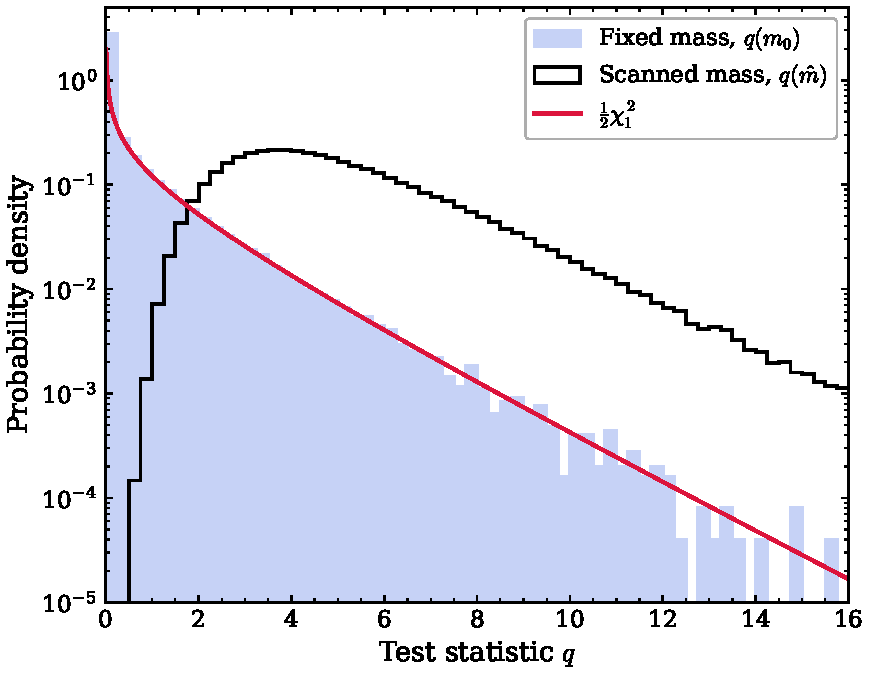
\includegraphics[width=0.48\textwidth]{figures/gg/q_null_dist.pdf}\hfill
    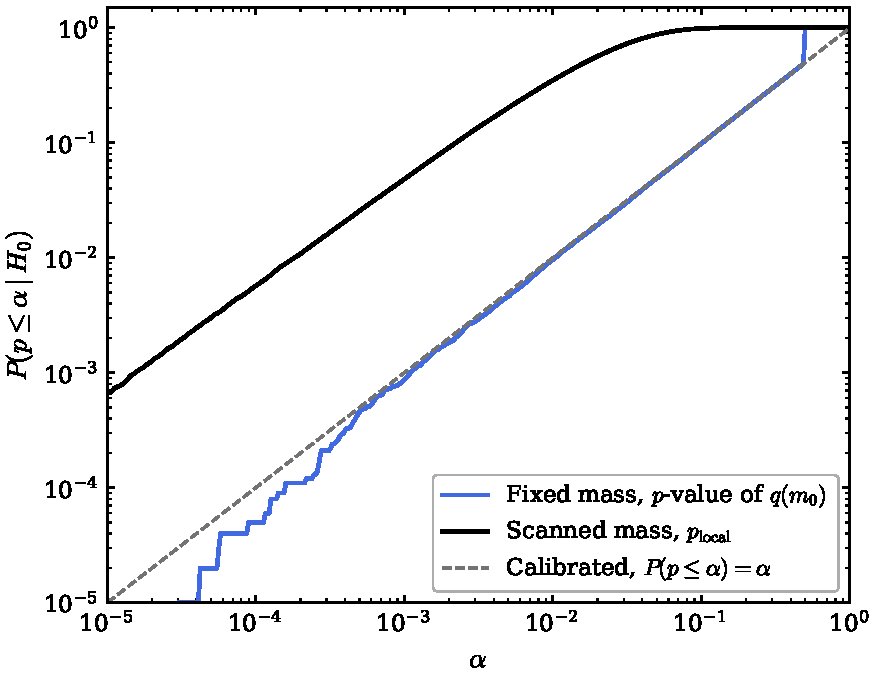
\includegraphics[width=0.48\textwidth]{figures/gg/pval_dist.pdf}
    %\caption{Left: Distribution of the test statistic for background-only toys, evaluated at a single fixed mass, $q(m_0)$, and as the maximum over the scanned range, $q(\hat{m})=\max_m q(m)$, compared with the asymptotic $\chi^2$ prediction. Right: Corresponding $p$-values, computed from the asymptotic $\chi^2$ tail probability.}
    \caption{Left: distribution of the test statistic in background-only pseudo-experiments, evaluated at a fixed mass, $q(m_0)$ with $m_0=3$ ($10^5$ pseudo-experiments), and at the best-fit mass, $q(\hat m)=\max_m q(m)$ ($3\times10^5$ pseudo-experiments, scan over $350$ mass points), compared with the asymptotic $\tfrac12\chi^2_1$ density. The first bin includes the entries with $q=0$. Right: fraction of pseudo-experiments with a $p$-value below $\alpha$, for the $p$-value of the fixed-mass statistic and for the local $p$-value $p_\text{local}$, both obtained from the asymptotic $\tfrac12\chi^2_1$ tail probability. The dashed line shows the expectation for a calibrated $p$-value, $P(p\leq\alpha)=\alpha$.}
    \label{fig:assym_q}
\end{figure}

\subsubsection{Trials factor estimation}\label{sec:exp_tf}
The trials factor is the ratio $p_\text{global}/p_\text{local}$, where $p_\text{global}=P(q(\hat m)>c\,|\,H_0)$ and $p_\text{local}=\tfrac12P(\chi^2_1>c)$ for an observed value $c$ of $q(\hat m)$. Estimating $p_\text{global}$ directly from pseudo-experiments is computationally expensive when $c$ is large. A global significance of $5\sigma$ requires $\mathcal{O}(10^7)$ toys. The Gross--Vitells (GV) procedure of Section~\ref{sec:gv} avoids this. It counts the upcrossings of a low reference level $c_0$ by $q(m)$, whose expected number $\langle N(c_0)\rangle$ can be estimated from a small number of toys, and extrapolates to the level of interest with Eq.~\eqref{eq:gv_extrapolation}. For the one-sided test statistic of Eq.~\eqref{eq:qmu}, with one fitted signal parameter ($s=1$), this gives
\begin{equation}
  p_\text{global}\approx p_\text{local}+\langle N(c_0)\rangle\,e^{-(c-c_0)/2}.
  \label{eq:gv_onesided}
\end{equation}
The left panel of Figure~\ref{fig:upcrossings-trials_factor} shows the upcrossings of $c_0=0.5$ in a background-only toy.
Although this pseudo-dataset contains no signal, its largest excursion, at $m=7.7$, reaches $q\approx4.5$, a local significance of $2.1\,\sigma$; once the look-elsewhere effect is accounted for with Eq.~\eqref{eq:gv_onesided}, no significant excess remains (global $p$-value $\approx0.6$).
%Estimating the null distribution of $q(\hat{m})$ from pseudo-experiments can be very computationally expensive, especially when the observed significance is high, since many toys are needed to populate the tail. In those cases, the Gross and Vitells procedure can be a useful alternative to estimate the trials factor. It relies on the expected number of upcrossings of a low reference level $c_0$ by the test statistic, which can be estimated from a small number of toys and then extrapolated to the level of interest $c$. In the left panel of Figure~\ref{fig:upcrossings-trials_factor} we illustrate the upcrossings over $c_0=0.5$ for background-only toys.

\begin{figure}[htbp]
    \centering
    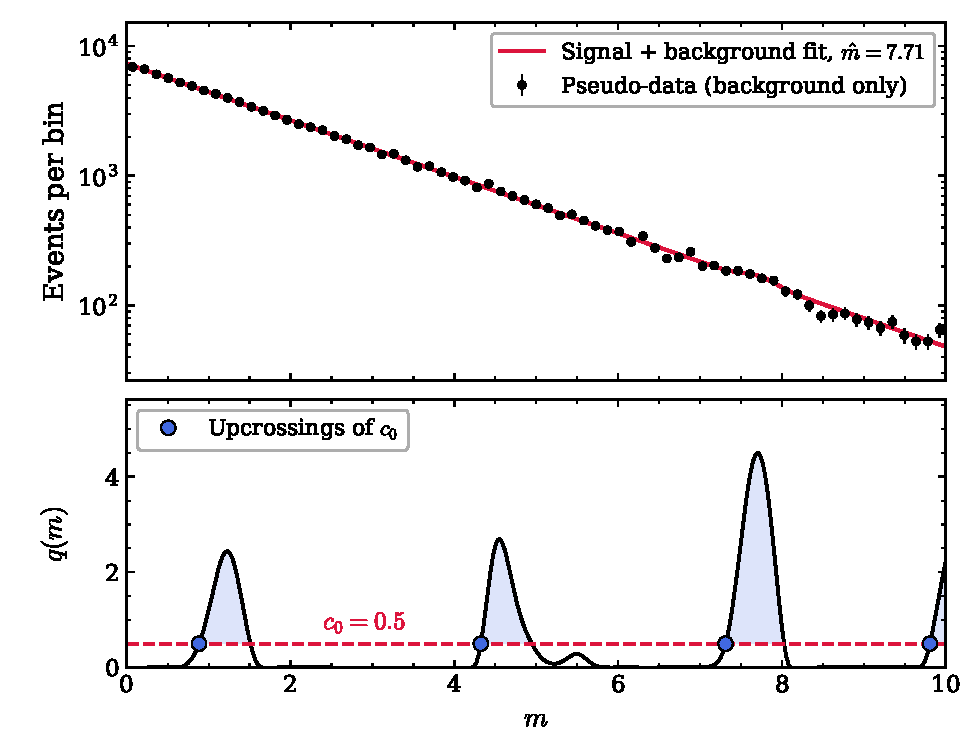
\includegraphics[width=0.49\textwidth]{figures/gg/mu_scan_upcrossings.pdf}
    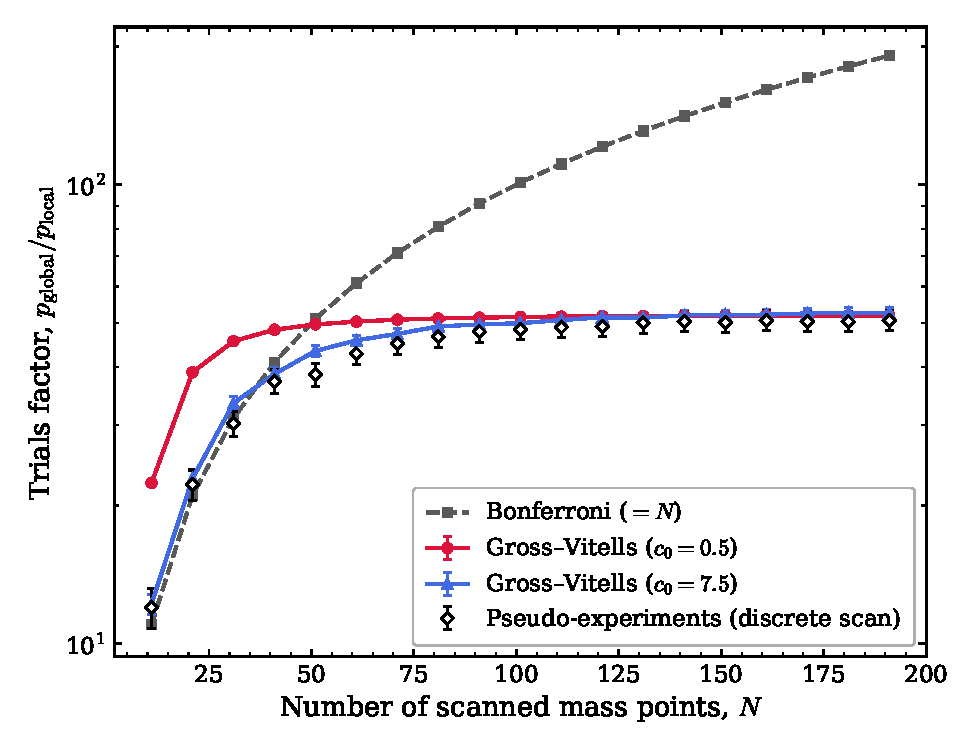
\includegraphics[width=0.49\textwidth]{figures/gg/trial_factor_Gv_Bon.pdf}
    \caption{Left: a background-only pseudo-dataset with the fit of $f(x|\mu, m,\nu)$ at the best-fit mass $\hat m=7.7$ (top), and the corresponding test statistic $q(m)$ on the 350-point grid (bottom), whose upcrossings of the reference level $c_0=0.5$ (dashed red line, circles) are counted in the GV procedure: four in this pseudo-dataset, compared with $\langle N(c_0)\rangle\approx4.6$ on average; a similar illustration is given in Ref.~\cite{gross2010}. Right: trials factor at $c=10$ as a function of the number $N$ of equally spaced mass points in the scan, for the Bonferroni bound ($=N$), for the GV procedure with $c_0=0.5$ and $c_0=7.5$, and for the discrete scan, estimated directly from the fraction of pseudo-experiments with $\max_i q(m_i)\geq c$ (open diamonds). All estimates use the same $10^4$ background-only pseudo-experiments.}
    \label{fig:upcrossings-trials_factor}
\end{figure}

The right panel of Figure~\ref{fig:upcrossings-trials_factor} shows how the trials factor depends on the number $N$ of equally spaced mass points in the scan. Two different quantities must be distinguished here. The first is the trials factor of the discrete scan, $P\big(\max_{i=1,\dots,N} q(m_i)>c\,\big|\,H_0\big)/p_\text{local}$, which is the relevant one for an analysis that evaluates $q(m)$ only at the $N$ grid points. It grows with $N$ and, since $p_\text{global}\leq N\,p_\text{local}$ for any $N$ tests, never exceeds the Bonferroni value $N$. The second is the trials factor of the continuous scan, the limit of the first as the grid becomes infinitely dense, which is what the GV procedure is designed to estimate. Toys analysed on the $N$-point grid estimate the former (open diamonds in the figure). The GV procedure, applied on the same grid, approaches the latter, and becomes independent of $N$, once the grid is dense enough to resolve every upcrossing of $c_0$. Two regimes can be distinguished:
%The Gross and Vitells procedure offers a much tighter bound on the trials factor than the simpler Bonferroni correction. Whereas the Bonferroni bound grows linearly with the number of scanned $m$ points $N$, the Gross-Vitells trials factor does not change with $N$ once the $m$ grid is dense enough to capture all the upcrossings over the selected reference level. In the right panel of Figure~\ref{fig:upcrossings-trials_factor} we show the trials factor as a function of the number of scanned $m$ points, for both the Bonferroni and Gross-Vitells procedures. Two regimes can be distinguished:
\begin{itemize}
    \item {\bf Coarse grid.} When the grid spacing is larger than the width of the peaks of $q(m)$, which is set by the width of the signal template, the scanned points are effectively independent tests. The trials factor of the discrete scan is then close to $N$, and the Bonferroni value is an accurate estimate of it. The GV estimate is not, because the extrapolation in Eq.~\eqref{eq:gv_onesided} assumes a smooth process: near a peak of a smooth $q(m)$, maximising over $m$ adds one degree of freedom, which is the origin of the $\chi^2_{s+1}$ term in Eq.~\eqref{eq:gv_asymptotic}. A set of independent points lacks this extra degree of freedom, so its tail falls faster with $c$ than the extrapolation assumes. Because the GV procedure measures the upcrossing rate at $c_0$ and rescales it to $c$, this mismatch grows with the gap between the two levels: the further $c$ lies above $c_0$, the more the GV estimate overshoots the trials factor of the discrete scan. For independent points, about $18\%$ of the steps of the scan upcross $c_0=0.5$, and extrapolating this rate to $c=10$ gives an estimate of about $1+2N$, roughly twice the trials factor of the discrete scan. This is the behaviour of the $c_0=0.5$ curve at small $N$, which lies above the Bonferroni line. For $c_0=7.5$ the extrapolation is short, and the GV estimate follows the Bonferroni value, but it requires a denser scan in order to correctly approximate the trials factor of the continuous scan.
    %\item {\bf Coarse grid:} When the number of scanned points $N$ is small, the spacing between neighbouring values of $m$ is much larger than the width of the peaks of $q(m)$, which is set by the width of the Gaussian signal template in the profile likelihood. Each scanned point then behaves as an effectively independent test. In this regime the Bonferroni bound estimates the trials factor well. The Gross-Vitells estimate, however, relies on counting the upcrossings of $c_0$, and on a coarse grid $q(m)$ may be sampled too sparsely to count them correctly. This can happen in two ways. If $c_0$ is too low, upcrossings are separated by less than the grid spacing and cannot be resolved, so they are undercounted. This is the case for $c_0=0.5$, where the Gross-Vitells extrapolation is unreliable. If $c_0$ is higher, as for $c_0=7.5$, the upcrossings are far enough apart to be resolved, but the excursions above $c_0$ are narrow, and one can fall between two scanned points and be missed. The Gross-Vitells estimate then agrees with the Bonferroni bound, but it has not yet reached its stable value.
    \item {\bf Dense grid.} When the grid spacing is smaller than both the distance between consecutive upcrossings and the width of the excursions above $c_0$, every upcrossing is resolved and counted. The GV estimate then no longer depends on $N$: it estimates the trials factor of the continuous scan, which is much smaller than the Bonferroni value. The value of $N$ needed to reach this regime depends on $c_0$. The excursions above $c_0$ narrow as $c_0$ increases (see the left panel of Figure~\ref{fig:upcrossings-trials_factor}), so a higher reference level requires a denser grid. In this example, the GV estimate is within $5\%$ of its dense-grid value for a grid spacing of about $1\,\sigma$ with $c_0=0.5$, and of about $0.5\,\sigma$ with $c_0=7.5$.
    %\item {\bf Dense grid:} When $N$ is large enough, the grid spacing is smaller than both the distance between consecutive upcrossings and the width of the excursions above $c_0$, so every upcrossing is resolved and counted. In this regime the Gross-Vitells estimate is stable with respect to $N$ and gives a much tighter bound on the trials factor than the Bonferroni correction. The value of $N$ required to reach this regime depends on $c_0$, because the width of an excursion shrinks as the reference level increases (see the left panel of Figure~\ref{fig:upcrossings-trials_factor}). A higher reference level therefore requires a denser grid to resolve the excursions. This is why $c_0=0.5$ reaches the stable regime at a smaller $N$ than $c_0=7.5$.
\end{itemize}

The GV procedure has two practical advantages when the level of interest $c$ is high. First, $\langle N(c_0)\rangle$ is estimated at a low level, where almost every toy contributes, so far fewer toys are needed than to populate the tail at $c$. Second, the intervals of $m$ in which $q(m)$ exceeds a low level $c_0$ are wider than those in which it exceeds a high level $c$, since only the tips of the tallest peaks rise above $c$. A grid fine enough to resolve the former is reached at a smaller $N$, so the GV estimate stabilises on a coarser grid than any method that works directly at $c$. Table~\ref{tab:trial_factors} quantifies both advantages at $c=10$, comparing three estimates of the trials factor obtained from the same pseudo-experiments: the Davies bound of Eq.~\eqref{eq:davies_bound}, with $\langle N(c)\rangle$ obtained by counting upcrossings directly at $c$; the GV estimate of Eq.~\eqref{eq:gv_onesided} with $c_0=0.5$; and the fully empirical estimate, given by the fraction of toys with $q(\hat m)>c$. The table also reports the estimate of Bayer and Seljak, which uses no pseudo-experiments and is discussed in Section~\ref{sec:exp_bayes}. On the 350-point grid, with a spacing of $\sigma/7$, the Davies and empirical estimates agree to within $1.5\%$, so the discrete scan is already close to the continuous limit. The GV estimate is a few per cent higher: between $c_0$ and $c$ the expected number of upcrossings falls slightly faster than the asymptotic factor $e^{-(c-c_0)/2}$ of Eq.~\eqref{eq:gv_onesided}, so that the extrapolation is slightly conservative in this example. 
% NOTE: with the three replicas of the table (3x10^5 toys) the number of upcrossings at c=10 is (4.3+-0.9)% below the
% GV extrapolation and GV is 4-6% above Davies/empirical. A fourth, independent sample of 10^5 toys (same code, seed
% 12345) gave empirical 52.88+-0.80 and Davies 53.59+-0.81, 4.6 sigma above the replicas; with all 4x10^5 toys the
% values are empirical 50.1+-0.4, Davies 50.8+-0.4, i.e. GV 2.5-4% higher. Hence 'a few per cent' in the text.
On the 100-point grid, with a spacing of $\sigma/2$, the GV estimate changes by only $1\%$, whereas the Davies and empirical estimates are both lower by about $6\%$, because the grid does not fully resolve the narrow peaks of $q(m)$ above $c$. The empirical value estimates the trials factor of the 100-point discrete scan, which is the relevant one for an analysis performed on that grid; for such an analysis, the GV estimate is conservative by about $10\%$. The GV estimate is also the most precise: with the same pseudo-experiments, its statistical uncertainty is about twenty times smaller than that of the Davies and empirical estimates, since the reference level $c_0$ is crossed in almost every toy, whereas the level $c$ is crossed in fewer than one toy in twenty.
%Therefore, the advantage of the Gross-Vitells procedure for computing the trials factor at high reference levels is twofold: it requires much fewer toys to estimate the number of upcrossings, and it needs less scanned points to reach the stable value of the trials factor. Both have a direct impact on the computational cost of estimating the global $p$-value. In Table~\ref{tab:trial_factors} we show the trials factor at $c=10$ for two different densities of the mass grid, computed using the Davies bound, the Gross-Vitells procedure, and the fully empirical Monte Carlo toys approach. The results are consistent within uncertainties, and they illustrate the advantages of the Gross-Vitells procedure over the other two methods.

\begin{table}[htbp]
    \centering
    \caption{Trials factor at $c=10$ estimated with four methods on two grids of equally spaced mass points. The first three use the same $3\times10^5$ background-only pseudo-experiments. The Davies and fully empirical estimates refer to the discrete scan on each grid, and the GV estimate to the continuous scan (see text). Their uncertainties are statistical: for the Davies and GV values they are propagated from the uncertainty on the mean number of upcrossings, and for the empirical value they are binomial, from the fraction of pseudo-experiments with $q(\hat{m})\geq c$. The Bayer--Seljak estimate (Section~\ref{sec:exp_bayes}) is computed for each dataset from the curvature of $q(m)$ at its maximum; the table gives its average over the pseudo-experiments with $|q(\hat m)-c|<2$, rescaled to $q(\hat m)=c$, with the statistical uncertainty on the average and, in brackets, the standard deviation between pseudo-experiments, which is the uncertainty of the estimate in a single analysis.}
    \label{tab:trial_factors}
    \begin{tabular}{lccc}
        \toprule
        Method & $N_\text{toys}$ & \multicolumn{2}{c}{Grid points (spacing)} \\
        \cmidrule(lr){3-4}
         & & 100 ($\sigma/2$) & 350 ($\sigma/7$) \\
        \midrule
        Davies, Eq.~\eqref{eq:davies_bound} & $3\times10^5$ & $47.02 \pm 0.44$ & $49.92 \pm 0.45$ \\
        GV, Eq.~\eqref{eq:gv_onesided}, $c_0=0.5$ & $3\times10^5$ & $51.53 \pm 0.02$ & $52.09 \pm 0.02$ \\
        Fully empirical & $3\times10^5$ & $46.48 \pm 0.44$ & $49.21 \pm 0.45$ \\
        Bayer--Seljak, Eq.~\eqref{eq:bs_exp} & -- & $51.16 \pm 0.06$ ($\pm10$) & $52.33 \pm 0.06$ ($\pm10$) \\
        \bottomrule
    \end{tabular}
\end{table}

\subsubsection{An estimate without pseudo-experiments}\label{sec:exp_bayes}
Section~\ref{sec:bayes} showed that the trials factor can also be obtained from a Bayesian argument, as the ratio of the prior to the posterior volume of the signal location~\cite{Bayer:2020pva}. In this example the prior range is the scan range, $U-L=10$, and the posterior width $\sigma_m$ is the precision with which the data localise the largest excess, which follows from the curvature of $q(m)$ at its maximum, $-\tfrac12\,q''(\hat m)=1/\sigma_m^2$. The trials factor and the global $p$-value are then
\begin{equation}
  N_B=\frac{U-L}{\sqrt{2\pi}\,\sigma_m},\qquad
  p_\text{global}\approx1-\exp\!\Big(-N_B\,\frac{e^{-q(\hat m)/2}}{\sqrt{2\pi\,q(\hat m)}}\Big),
  \label{eq:bs_exp}
\end{equation}
where, as in Ref.~\cite{Bayer:2020pva}, the local $p$-value is used in its asymptotic form.\footnote{With this form, $N_B$ times the local $p$-value equals the second term of the Davies bound, Eq.~\eqref{eq:davies_normal}, in which the oscillation rate of the process is estimated from the curvature of the observed peak. With the exact local $p$-value, $\tfrac12P(\chi^2_1>c)$, the estimate at $c=10$ would be about $8\%$ lower.} Both quantities are computed from the observed dataset alone: no pseudo-experiments are needed. We compute $q''(\hat m)$ by repeating the fit at $\hat m\pm0.02$, so that the estimate does not depend on the spacing of the scan.

To assess its accuracy, we apply Eq.~\eqref{eq:bs_exp} to each of the background-only pseudo-experiments of Table~\ref{tab:trial_factors}. On average, the Bayer--Seljak trials factor at $c=10$ agrees with the GV estimate to within $1\%$ on both grids, and, like it, lies a few per cent above the Davies and empirical estimates on the 350-point grid. The agreement with GV is expected. Near a high peak of local significance $Z$, the posterior width is $\sigma_m=1/(Z\sqrt{-\rho_{11}})$, so that $N_B$ reproduces the leading term of the Davies bound, and both estimate the same oscillation rate of the process: the value of $\sqrt{-\rho_{11}}$ inferred from the curvature of the peaks, $3.66$, agrees to within 2\% with that inferred from the upcrossing rate measured in the GV procedure, $3.73$.

The two approaches differ in what they average. The GV and Davies estimates average the upcrossing rate over many pseudo-experiments, whereas $N_B$ is estimated from the single observed peak, whose curvature fluctuates from one dataset to the next. The left panel of Figure~\ref{fig:bs} shows the trials factor as a function of the local significance. The Bayer--Seljak estimate follows the growth with $Z_\text{local}$ of the GV extrapolation and of the pseudo-experiments, but individual datasets scatter around it by about 20\% for local significances between $2.5$ and $4\,\sigma$. Below about $2.5\,\sigma$ it also follows the pseudo-experiments, where the GV formula, an approximation for the tail, overestimates the trials factor; this is because Eq.~\eqref{eq:bs_exp} has the form of a \v{S}id\'ak correction, which remains below one. The right panel compares, dataset by dataset, the estimated global $p$-values with those obtained from the full set of pseudo-experiments. The GV $p$-value is a fixed function of $q(\hat m)$ and lies on a single curve, whereas the Bayer--Seljak $p$-values scatter around the diagonal. The scatter averages out over the pseudo-experiments: the Bayer--Seljak $p$-value is below $\alpha$ in a fraction $0.050$ of them for $\alpha=0.05$ and $0.010$ for $\alpha=0.01$, so that it is correctly calibrated as a test.\footnote{For the right panel we follow the prescription of Ref.~\cite{Bayer:2020pva}, which selects, among all local maxima of $q(m)$, the one with the largest value of $-2\ln p_\text{global}$; in most datasets this is the highest peak.}

The Bayer--Seljak estimate thus provides, from a single fit around the observed excess, the trials factor of the continuous scan with an accuracy of about 20\%, which corresponds to a shift of less than $0.1\,\sigma$ in the global significance at the discovery level.\footnote{At $Z_\text{local}=5$, $p_\text{local}=2.9\times10^{-7}$; the GV trials factor of this example, $78$, gives $Z_\text{global}=4.08$, and a trials factor $20\%$ larger or smaller gives $4.04$ or $4.13$.} Its limitations are those of the asymptotic regime on which it relies (Section~\ref{sec:bayes}): it requires a smooth, approximately Gaussian likelihood and a high peak, and it uses the width of the observed peak to represent the whole scan range, which would be inaccurate if the resolution varied strongly across the range. Like the GV procedure, it does not apply to the machine-learning test statistics of Section~\ref{sec:ml}.
% NOTE: \ref{sec:ml} is a guess for the label of Section 6; please adjust.

\begin{figure}[htbp]
    \centering
    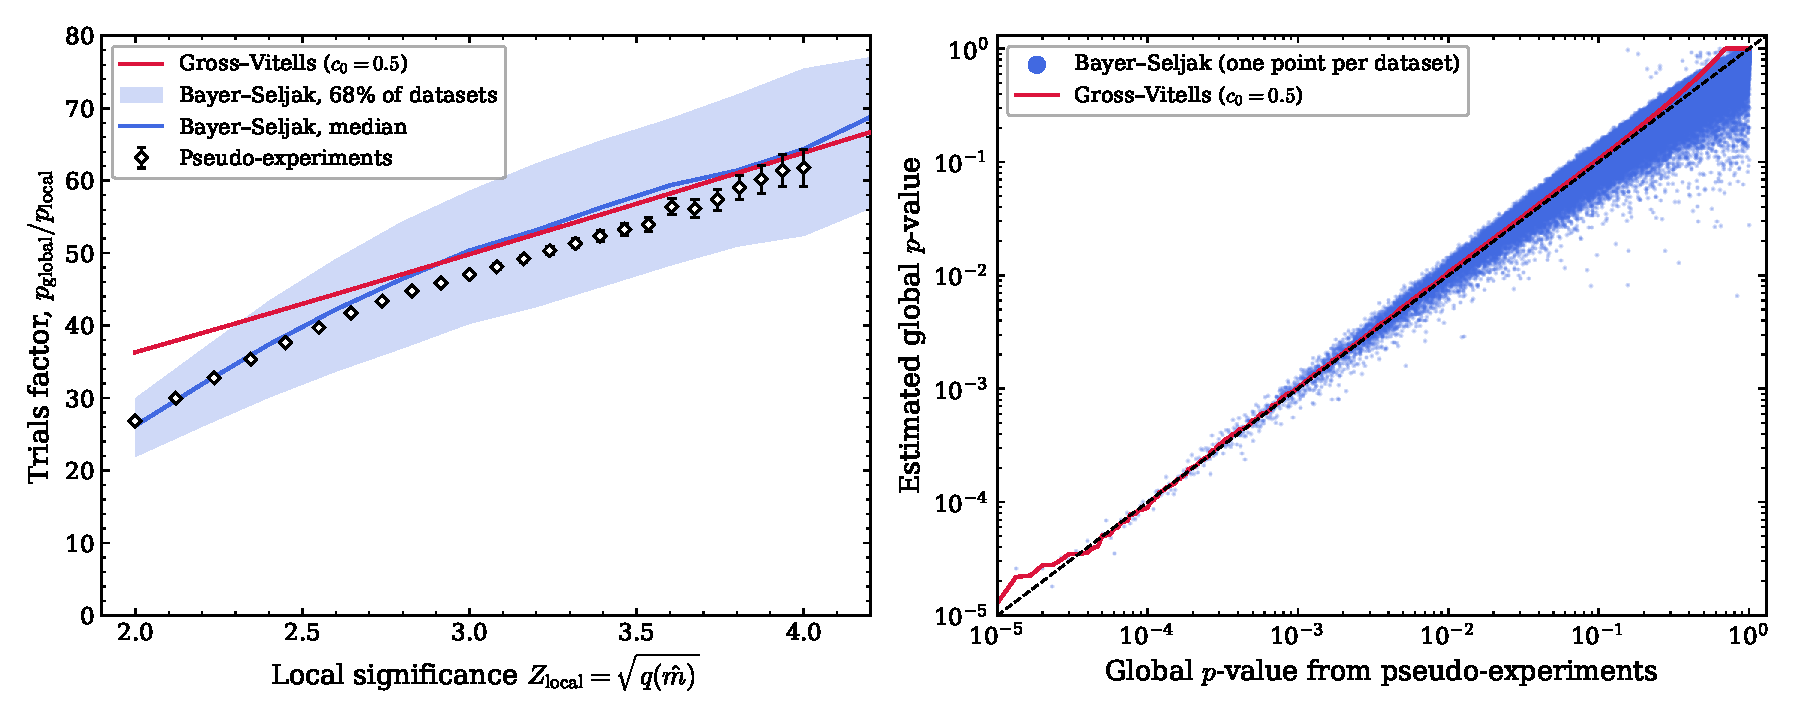
\includegraphics[width=\textwidth]{figures/gg/bs_comparison.pdf}
    \caption{Comparison of the Bayer--Seljak estimate, Eq.~\eqref{eq:bs_exp}, computed from each dataset without pseudo-experiments, with the GV procedure and with the pseudo-experiments, for the 350-point scan. Left: trials factor as a function of the local significance of the highest peak, $Z_\text{local}=\sqrt{q(\hat m)}$, from the fraction of pseudo-experiments above each level (open diamonds), from the GV extrapolation with $c_0=0.5$ (red line), and from the Bayer--Seljak estimate of each dataset (median and central $68\%$ of the datasets in bins of $Z_\text{local}$, blue). Right: global $p$-value of each dataset estimated with the Bayer--Seljak method (one point per dataset) and with the GV procedure (red line), as a function of the global $p$-value obtained from the full set of pseudo-experiments; the dashed line marks equality. Both panels use $3\times10^5$ background-only pseudo-experiments.}
    \label{fig:bs}
\end{figure}

\subsubsection{Dependence on the signal-template width}\label{sec:exp_width}
The width of the signal template used in the fit sets how rapidly $q(m)$ varies with $m$, and therefore how many upcrossings of a given reference level occur over the scan range. Figure~\ref{fig:width_dependence} shows the GV trials factor at $c=10$ as a function of the template width. Since the pseudo-experiments are background-only, their distribution does not depend on the width: only the template used in the fit changes. Broader templates produce $q(m)$ curves that vary more slowly with $m$, with fewer upcrossings and hence a smaller trials factor. This matches the intuition that the effective number of independent tests scales roughly as the ratio of the scan range to the template width. For widths comparable to the scan range, the signal shapes at different masses overlap almost entirely, so the tests at different masses are strongly correlated and the scan behaves almost like a single test: the trials factor approaches one (dashed line).
%The width of the signal template affects the shape of the test statistic $q(m)$, and therefore the number of upcrossings over a given reference level. In Figure~\ref{fig:width_dependence} we show the trials factor computed using the Gross-Vitells procedure as a function of the signal template width. Broader signal templates lead to $q(m)$ curves that vary more slowly with $m$, which results in fewer effectively independent excursions over a given reference level and therefore a smaller trials factor. This matches the intuition that the effective number of independent tests scales roughly as the ratio of the scanned range to the signal width. The trials factor saturates for very broad signals, where the test statistic becomes almost flat over the scanned range.

This intuition can be made quantitative with the Davies bound of Section~\ref{subsec:davies}. To apply it, we write the test statistic in terms of the signed square root of the likelihood ratio,
\begin{equation}
  Z(m)=\operatorname{sign}(\hat\mu_m)\sqrt{t(m)},\qquad
  t(m)=-2\ln\frac{\mathcal{L}(\mu=0,\,\hat{\hat{\nu}})}{\mathcal{L}(\hat\mu_m,\,\hat\nu_m;\,m)},
  \label{eq:Zm}
\end{equation}
where $t(m)$ is the likelihood ratio of Eq.~\eqref{eq:qmu}, evaluated for either sign of $\hat\mu_m$. Excesses give $Z(m)>0$ and deficits $Z(m)<0$, and the two statistics are related by $q(m)=Z(m)^2$ when $Z(m)>0$ and $q(m)=0$ otherwise. Under the null hypothesis, $Z(m)$ follows a standard normal distribution at each mass and, as a function of $m$, is asymptotically a Gaussian process with unit variance. It therefore plays the role of $S(\theta)$ in Eq.~\eqref{eq:davies_normal}, with $\theta\to m$ and $[L,U]=[0,10]$. Since $q(\hat m)>c$ exactly when $\max_m Z(m)>\sqrt{c}$, Eq.~\eqref{eq:davies_normal} is evaluated at the level $\sqrt{c}$. Its first term then becomes $\Phi(-\sqrt{c})=\tfrac12P(\chi^2_1>c)=p_\text{local}$, and its second term the expected number of upcrossings, $\langle N(c)\rangle=\mathcal{N}e^{-c/2}$, with $\mathcal{N}=\frac{1}{2\pi}\int_L^U\sqrt{-\rho_{11}(m)}\,dm$. For a Gaussian template, and neglecting the edges of the range and the fit of the background normalisation and slope, the correlation is $\rho(m',m)=\exp[-(m'-m)^2/4\sigma^2]$, independently of the exponential background,\footnote{Asymptotically, $Z(m)$ is proportional to the score $\int g(x\,|\,m,\sigma)\,[dn(x)-b(x)\,dx]/b(x)$, where $b(x)$ is the background density and $dn(x)$ the observed events, so that $\rho(m',m)$ is $\int g(x\,|\,m',\sigma)\,g(x\,|\,m,\sigma)/b(x)\,dx$ divided by the corresponding normalisations. For $b\propto e^{-\nu x}$, the factor $e^{\nu x}$ contributes the same factor $e^{\nu(m+m')/2+\nu^2\sigma^2/4}$ to the numerator and to the normalisation, and cancels.} so that $\rho_{11}=-1/(2\sigma^2)$ and
\begin{equation}
  \mathcal{N}=\frac{U-L}{2\sqrt{2}\,\pi\,\sigma}.
  \label{eq:N_analytic}
\end{equation}
This is the functional form of Eq.~\eqref{eq:gv_onesided}: the GV procedure measures the normalisation $\langle N(c_0)\rangle$ with toys, whereas here it is computed analytically. For $\sigma=0.2$, Eq.~\eqref{eq:N_analytic} gives $\mathcal{N}\approx5.6$ and $\langle N(c_0{=}0.5)\rangle\approx4.4$, compared with 4.6 measured with toys, and a trials factor of about 49 at $c=10$, about $5\%$ below the GV estimate on the dense grid in Table~\ref{tab:trial_factors}. More generally, Eqs.~\eqref{eq:gv_onesided} and~\eqref{eq:N_analytic} give the trials factor at any level $c$,
\begin{equation}
  \frac{p_\text{global}}{p_\text{local}}\approx1+\kappa(c)\,\frac{U-L}{\sigma},\qquad
  \kappa(c)=\frac{e^{-c/2}}{2\sqrt{2}\,\pi\,\Phi(-\sqrt{c})}.
  \label{eq:tf_analytic}
\end{equation}
This makes the familiar rule of thumb that the trials factor is the ratio of the scan range to the template width more quantitative. The rule captures the dependence on $\sigma$, while the prefactor $\kappa$ grows with the local significance $\sqrt{c}$, as in Eq.~\eqref{eq:trial_factor}. For local significances of $3$, $4$ and $5\,\sigma$, $\kappa\approx0.93$, $1.2$ and $1.5$, so the rule is numerically accurate only around $3\,\sigma$ and underestimates the trials factor at the discovery level.

Figure~\ref{fig:width_dependence} compares Eq.~\eqref{eq:tf_analytic} at $c=10$ with the GV estimates. The approximation is accurate for narrow templates, within $1\%$ at $\sigma=0.1$ and $5\%$ at $\sigma=0.2$. This is the regime of most resonance searches, in which the template is much narrower than both the scan range and the scale over which the background varies. For broader templates the GV points lie up to $40\%$ above the approximation, and fall below it only for $\sigma\gtrsim4$, after a sharp drop. The discrepancy does not come from the GV procedure but from the two simplifications behind Eq.~\eqref{eq:N_analytic}. First, the fit of the background absorbs the component of the signal template that mimics a change of the background normalisation or slope; for broad templates the remaining shape varies faster with $m$ than the template itself, and the number of upcrossings increases. Second, at the edges of the range the templates are truncated, which reduces the number of upcrossings for broad templates. Both effects are included if the correlation of the process is computed from the binned templates,
\begin{equation}
  \rho(m',m)=\frac{\langle w_{m'},w_m\rangle}{\lVert w_{m'}\rVert\,\lVert w_m\rVert},\qquad
  \langle u,v\rangle=\sum_i\frac{u_i\,v_i}{b_i},
  \label{eq:rho_binned}
\end{equation}
where $b_i$ is the background in bin $i$ and $w_m$ is the signal template $g(x_i\,|\,m,\sigma)$ minus its projection, with the same inner product, onto the directions absorbed by the background fit, $b_i$ and $\partial b_i/\partial\nu$. Evaluating $\mathcal{N}$ numerically with this correlation gives the solid black line, which agrees with the GV estimates to within $10\%$ for all widths, and within $5\%$ for $\sigma\lesssim2.5$, including the sharp drop near $\sigma\approx4$. This drop has a simple origin: for $1\lesssim\sigma\lesssim4$ there is a mass inside the scan range at which the template is almost entirely absorbed by the background fit, and around which the residual shape changes rapidly with $m$; as $\sigma$ increases, this mass moves towards the lower edge of the range, which it leaves at $\sigma\approx4.2$. Repeating the GV procedure with the background slope fixed to its true value (open points) removes the drop, and agrees with the corresponding Davies prediction, in which only the normalisation is projected out (solid blue line). The Davies/GV framework therefore describes the trials factor accurately for all widths, once the correlation of the process is computed for the actual fit; Eq.~\eqref{eq:tf_analytic} is a useful approximation for templates much narrower than the scan range and than the scale of the background.

\begin{figure}[h!]
    \centering
    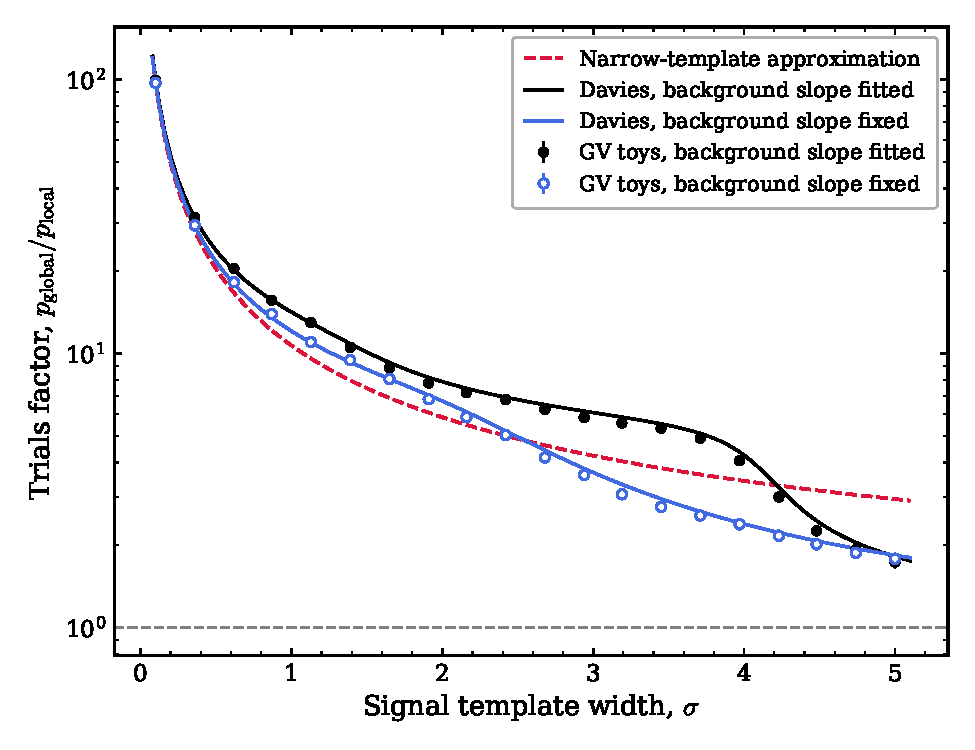
\includegraphics[width=0.6\textwidth]{figures/gg/tfactor_vs_signalwidth.pdf}
    \caption{Trials factor at $c=10$ as a function of the width $\sigma$ of the signal template used in the fit, from the GV procedure with $c_0=0.5$ applied to $1000$ background-only pseudo-experiments on a grid of $350$ mass points, with the background slope fitted (filled points) or fixed to its true value (open points). The red dashed line shows the narrow-template approximation of Eq.~\eqref{eq:tf_analytic}. The solid lines show the Davies prediction with the correlation of Eq.~\eqref{eq:rho_binned}, with the background slope fitted (black) or fixed (blue). The grey dashed line marks a trials factor of one.}
    \label{fig:width_dependence}
\end{figure}

This example shows explicitly that the LEE is not determined by the search range alone, but also by the signal model used in the scan: the background-only pseudo-experiments are the same for every width, and only the template used in the fit changes (Section~\ref{sec:model_dependence}). In many high-energy physics searches, the width of the template is set by the detector resolution, so the trials factor is set by the ratio of the scan range to the resolution.
In other cases, such as resonances of unknown intrinsic width, the width becomes a free parameter, and the scan extends over an additional dimension, which further increases the LEE (Section~\ref{sec:multidim}). Since the trials factor grows as $1/\sigma$, such a scan is dominated by its narrowest templates, and the lower end of the width range should be motivated physically, for example by the detector resolution, rather than chosen for convenience.
%This example shows explicitly that the LEE is not determined by the search range alone, but also by the signal model used in the scan. In many high-energy physics searches the width of the signal template is fixed by the detector resolution, so the trials factor is set by the ratio of the scanned range to the resolution. In other cases, such as wide resonances or searches for new physics in the tails of distributions, the width of the signal template can be a free parameter. The scan then extends over an additional dimension, which further increases the LEE. In those cases, the choice of signal template and its impact on the LEE should be considered carefully when designing a search for new physics.

\subsection{Multi-channel search}\label{subsec:exp2}
Many searches in high-energy physics involve several channels, for example different decay modes of the same particle, or event categories defined by detector region or by the number of reconstructed objects. In these cases, the LEE arises not only from the scan over the signal parameters within each channel, but also from the number of channels considered, which is case~(ii) of Section~\ref{sec:case_ii}. In this section, we illustrate how the multiple-testing corrections of Section~\ref{sec:multipletesting} handle this additional layer, and compare them with a combined fit across channels.
%In high energy physics, many searches for new physics involve multiple channels. This can be due to different decay modes of the same particle, or to different final states that can be produced by the same underlying process. In these cases, the LEE can arise not only from scanning over a range of parameters in each channel, but also from the fact that multiple channels are being considered simultaneously. In this section, we present two simple examples of multi-channel searches, and discuss how the LEE can be handled in these cases.

\subsubsection{Decay channels of a new particle}\label{sec:exp_decay}
We consider a resonance that decays into $N_\text{ch}=6$ channels with unknown branching ratios. Each channel is modelled as in Section~\ref{subsec:exp1}, by Eq.~\eqref{eq:toy_model} with its own background and signal fraction $\mu_i$. The resonance mass is unknown but common to all channels, while the width of the Gaussian signal template differs from channel to channel, reflecting the different detector resolution of each final state. The resonance is narrow: its intrinsic width, $\Gamma=0.02$, is much smaller than the resolutions $\sigma_i$, which range from $0.15$ to $0.40$, so that the observed signal in channel $i$ is a Gaussian of width $\sqrt{\Gamma^2+\sigma_i^2}\approx\sigma_i$, and each channel is fitted with a template of width $\sigma_i$. A signal at $m=3$ is injected in three channels, two with a strong and one with a weak signal, with signal fractions chosen to give an expected local significance of $4.5\,\sigma$ in channels~1 and~6 and of $3.5\,\sigma$ in channel~3;\footnote{The expected local significance is $\sqrt{q(m)}$ at the true mass for the Asimov dataset, in which the bin contents are equal to their expected values~\cite{Cowan:2010js}.} the remaining three contain background only. The parameters of each channel, together with the results of the per-channel scans in one pseudo-experiment, are listed in Table~\ref{tab:channels}.
\begin{table}[htbp]
  \centering
  \caption{Channels of the multi-channel example: number of events, background decay rate, template width (equal to the detector resolution) and injected signal fraction, followed by the best-fit mass, the maximum of the test statistic, and the GV-corrected global $p$-value of each channel, in one pseudo-experiment.}
  \label{tab:channels}
  \begin{tabular}{ccccc|ccc}
    \toprule
    Channel & $N_\text{ev}$ & $\nu$ & $\sigma$ & $\mu$ & $\hat m$ & $q(\hat m)$ & $p_\text{GV}$ \\
    \midrule
    1 & $10^5$ & 0.50 & 0.15 & 0.0037 & 3.04 & 24.9 & $3.1\times10^{-5}$ \\
    2 & $10^5$ & 0.30 & 0.25 & 0 & 1.95 & 3.3 & 0.96 \\
    3 & $10^5$ & 0.40 & 0.20 & 0.0035 & 2.81 & 21.1 & $1.6\times10^{-4}$ \\
    4 & $10^5$ & 0.20 & 0.40 & 0 & 0.72 & 2.7 & 0.90 \\
    5 & $10^5$ & 0.60 & 0.30 & 0 & 7.59 & 4.9 & 0.37 \\
    6 & $10^5$ & 0.35 & 0.35 & 0.0062 & 3.24 & 20.0 & $1.7\times10^{-4}$ \\
    \bottomrule
  \end{tabular}
\end{table}
We first treat each channel separately and ask which channels contain a signal. This is the per-channel formulation of Section~\ref{sec:multipletesting}, appropriate when a separate decision is required for each channel. The analysis has two levels, as in the hierarchical searches of Section~\ref{sec:case_ii}. Within each channel, the scan over the resonance mass is corrected with the GV procedure, which gives one global $p$-value per channel. The expected number of upcrossings $\langle N(c_0)\rangle$ is estimated separately for each channel, from $5000$ background-only pseudo-experiments generated with the background of that channel and fitted with its template; it ranges from $6.0$ for the narrowest template ($\sigma=0.15$) to $2.5$ for the broadest ($\sigma=0.40$), following the dependence on the template width discussed in Section~\ref{sec:exp_width}. Across channels, these $p$-values are then corrected for the number of channels. For this second level, we compare the Bonferroni and \v{S}id\'ak corrections, which control the family-wise error rate (Sec.~\ref{sec:bonferroni}), with the Benjamini--Hochberg (BH) procedure (Sec.~\ref{sec:bh}), which controls the false discovery rate. Since the channels are statistically independent, the \v{S}id\'ak correction is exact here. For illustration, we use a level $\alpha=0.05$ throughout, much looser than a discovery threshold in high energy physics.
%In this example, we consider a resonance decaying into $N_{ch}=6$ different channels, each with a different and unknown branching ratio. The signal template is the same used in the previous single-channel example, but now we have $N_{ch}$ independent channels, each with its own background and signal injection. The position of the resonance is unknown, but it is the same for all channels. On the other hand, the width of the signal template can change from channel to channel, reflecting the different detector resolutions for each final state. If we want to ask if there is a signal in any of the channels, we need to correct for the LEE arising from the multiple channels search. There are several ways to do this, depending on the assumptions we make about the signal model. In this example, we compare the Bonferroni, the Sidak, and the BH procedures, which are all based on the p-values of the individual channels, which already account for the LEE arising from the scan over the resonance position through the Gross-Vitells correction.
\begin{comment}
\begin{figure}[htbp]
    \centering
    \includegraphics[width=0.6\textwidth]{figures/global_pval_per_channel.pdf}
    \caption{Global $p$-value of each channel, corrected with the GV procedure for the scan over the resonance mass but not for the number of channels, using \textcolor{red}{[\dots]} background-only toys per channel. Channels with an injected signal are marked with stars, and the dashed line indicates $\alpha=0.05$.}
    \label{fig:decay-global}
\end{figure}

\begin{figure}[h]
    \centering
    \includegraphics[width=0.28\textwidth]{figures/bonferroni_corrected_pval.pdf}
    \includegraphics[width=0.30\textwidth]{figures/sidak_corrected_pval.pdf}
    \includegraphics[width=0.28\textwidth]{figures/bh_corrected_pval.pdf}
    \caption{Multi-channel corrections applied to the $p$-values of Figure~\ref{fig:decay-global}. Left and centre: Bonferroni-adjusted, $\min(1,N_\text{ch}\,p)$, and \v{S}id\'ak-adjusted, $1-(1-p)^{N_\text{ch}}$, $p$-values of each channel, compared with $\alpha=0.05$ (dashed line). Channels with a signal that are identified (true positives) are shown in green, missed ones (false negatives) in red, and background-only channels in grey. Right: $p$-values sorted by rank $k$, compared with the BH threshold $k\alpha/N_\text{ch}$ for a false discovery rate of $0.05$.}
    \label{fig:decay-corrected}
\end{figure}
Figure~\ref{fig:decay-global} shows the $p$-value of each channel after the Gross--Vitells correction for the scan over the resonance position, but before any correction for the number of channels. Figure~\ref{fig:decay-corrected} shows the results after applying the three multi-channel procedures. All three lead to the same decisions: the two strong signal channels are detected and the weak one is missed. This is expected for several reasons. First, the \v{S}id\'ak and Bonferroni corrections agree to first order in $p$, so for small $p$-values and a modest number of channels they are almost identical. Second, BH gives a different result from Bonferroni only for $p$-values that fall within a narrow window above $\alpha/N_{\mathrm{ch}}$. Here the strong channels lie well below that window and the weak channel lies well above it. Finally, the within-channel trials factor is much larger than the multi-channel one, so most of the correction comes from the look-elsewhere effect inside each channel and not from how the channels are combined.

More fundamentally, these procedures answer the question of \emph{which} channels contain a signal, whereas claiming the discovery of a single resonance requires a single global $p$-value. The most common alternative in high-energy physics is to build a combined likelihood, given by the product of the likelihoods of the individual channels, with a single mass $m$ shared by all channels. Since the branching ratios are unknown, each channel keeps its own free signal strength $\mu_i$. Therefore the look-elsewhere correction is applied only once, to $\max_m q_{\mathrm{comb}}(m)$. This approach is more powerful because channels with weak individual excesses can still contribute if they occur at the same mass. In our example, $\sum_i \max_m q_i(m)\simeq 42$, compared with $16.4$ for the best single channel. This sum is only an upper bound on $\max_m q_{\mathrm{comb}}(m)$, since the individual channels peak at slightly different values of $m$, but it illustrates the potential gain of the combination.
\end{comment}

\begin{figure}[htbp]
    \centering
    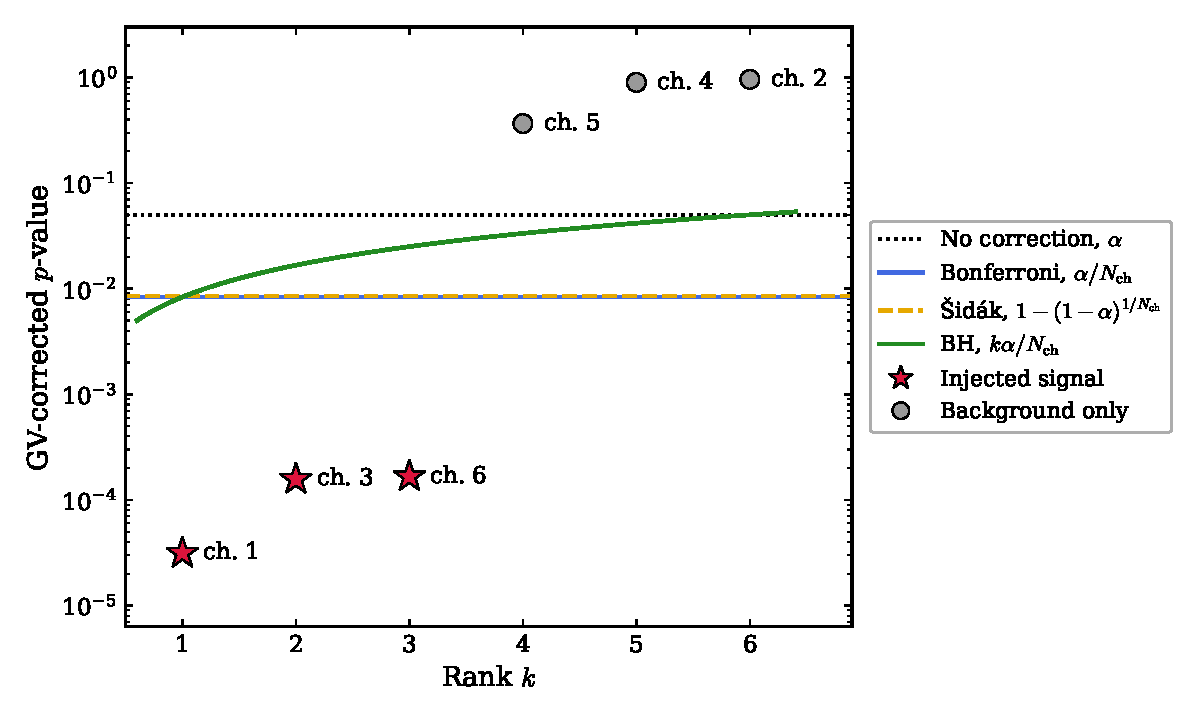
\includegraphics[width=0.85\textwidth]{figures/gg/multichannel_thresholds.pdf}
    \caption{Global $p$-values of the six channels in one pseudo-experiment, corrected with the GV procedure for the scan over the resonance mass, using $5000$ background-only toys per channel, but not for the number of channels. The $p$-values are sorted in increasing order and labelled by channel number. Stars mark channels with an injected signal, and circles background-only channels. The horizontal lines show the per-channel thresholds without correction ($\alpha=0.05$), and with the Bonferroni ($\alpha/N_\text{ch}$) and \v{S}id\'ak ($1-(1-\alpha)^{1/N_\text{ch}}$) corrections, which are indistinguishable on this scale. The rising line shows the BH threshold $k\alpha/N_\text{ch}$. Bonferroni and \v{S}id\'ak identify every channel whose $p$-value lies below their threshold; BH identifies all channels up to the largest rank $k$ whose $p$-value lies below its line. The error rates of the three procedures over many pseudo-experiments are given in Table~\ref{tab:channel_rates}.}
    \label{fig:decay-pvalues}
\end{figure}

Figure~\ref{fig:decay-pvalues} shows the global $p$-value of each channel after the GV correction for the scan over the resonance mass, sorted in increasing order, together with the uncorrected level $\alpha$ and the per-channel thresholds of the three multi-channel procedures. The background-only channels have large $p$-values, between $0.37$ and $0.96$, as expected for background fluctuations once the look-elsewhere effect within each channel is accounted for. The three channels with a signal lie below every threshold and are identified by all three procedures, and no background-only channel is selected. In this pseudo-experiment, an upward fluctuation brings the weak signal of channel~3 to a significance similar to that of channel~6.

The figure also shows why the three procedures lead to the same decisions here. For six channels, the Bonferroni and \v{S}id\'ak thresholds, $8.33\times10^{-3}$ and $8.51\times10^{-3}$, differ by only $2\%$, since the two corrections agree to first order in $\alpha$, and their lines coincide on the scale of the figure. The BH threshold starts at the Bonferroni value for the smallest $p$-value and rises linearly with the rank $k$, reaching the uncorrected level $\alpha$ at $k=N_\text{ch}$: BH interpolates between the Bonferroni correction and no correction at all. It identifies more channels than Bonferroni only if, for some $k>1$, the $k$-th smallest $p$-value lies between $\alpha/N_\text{ch}$ and $k\alpha/N_\text{ch}$. Here, the three signal channels lie below $\alpha/N_\text{ch}$ and the background-only channels above $\alpha$, so that no $p$-value falls in such an interval. Had the third-ranked $p$-value fallen between $8.3\times10^{-3}$ and $3\alpha/N_\text{ch}=0.025$, BH would have identified that channel, while the Bonferroni and \v{S}id\'ak corrections would not. The procedures differ substantially only when many channels fall in such intervals, as in the screening regime with many channels and several signals discussed in Section~\ref{sec:bh}.

A single pseudo-experiment cannot show the error rates that the procedures control, which are averages over repeated experiments. Table~\ref{tab:channel_rates} reports them for $5000$ pseudo-experiments generated with the same configuration: the family-wise error rate (FWER), i.e.\ the fraction of pseudo-experiments in which at least one background-only channel is selected; the false discovery rate (FDR), i.e.\ the average fraction of background-only channels among the selected ones; and the fraction of pseudo-experiments in which each signal channel is identified. Without a correction for the number of channels, at least one of the three background-only channels is selected in $14\%$ of the pseudo-experiments, close to $1-(1-\alpha)^3$. The Bonferroni and \v{S}id\'ak corrections reduce this to $2.3\%$: since only $N_0=3$ of the six null hypotheses are true, the bound on the FWER is $N_0\alpha/N_\text{ch}=0.025$ rather than $\alpha$. BH controls the FDR at the same level, $N_0\alpha/N_\text{ch}=0.025$, which it reaches here, but lets the FWER rise to $8\%$, above $\alpha$. In exchange, it identifies the weak signal of channel~3 in $63\%$ of the pseudo-experiments, compared with $50\%$ for Bonferroni, and the strong signals in about $90\%$ instead of $85\%$. This is the trade-off discussed in Section~\ref{sec:bh}: FWER control is the appropriate criterion for a discovery claim, and FDR control for a screening stage in which a controlled fraction of false leads is acceptable.
\begin{table}[htbp]
  \centering
  \caption{Error rates and identification probabilities of the multi-channel procedures at $\alpha=0.05$, from $5000$ pseudo-experiments of the six-channel example: family-wise error rate (FWER), false discovery rate (FDR), and fraction of pseudo-experiments in which each signal channel is identified. The statistical uncertainties are below $0.005$ for the FWER, $0.002$ for the FDR and $0.007$ for the identification probabilities.}
  \label{tab:channel_rates}
  \begin{tabular}{lccccc}
    \toprule
    Procedure & FWER & FDR & \multicolumn{3}{c}{Identification rate} \\
    \cmidrule(lr){4-6}
     & & & ch.~1 & ch.~3 & ch.~6 \\
    \midrule
    No correction & 0.139 & 0.041 & 0.93 & 0.72 & 0.96 \\
    Bonferroni & 0.023 & 0.008 & 0.82 & 0.50 & 0.87 \\
    \v{S}id\'ak & 0.023 & 0.008 & 0.83 & 0.50 & 0.87 \\
    BH & 0.082 & 0.025 & 0.88 & 0.63 & 0.92 \\
    \bottomrule
  \end{tabular}
\end{table}

The example also shows where most of the correction comes from. For the most significant channel, channel~1, with $q(\hat m)=24.9$, the trials factor of the mass scan is about $100$, much larger than the factor $N_\text{ch}=6$ across channels, so the look-elsewhere effect inside each channel dominates the total correction. The trials factor also differs between channels: for channel~6, with a similar $q(\hat m)=20.0$ but a template more than twice as broad, it is about $40$.

More fundamentally, these procedures answer the question of \emph{which} channels contain a signal, whereas claiming the discovery of a single resonance requires a single global $p$-value. The most common approach in high-energy physics is a combined likelihood, given by the product of the likelihoods of the individual channels, with a single mass $m$ shared by all channels. Because $m$ is shared, the scan, and hence the look-elsewhere correction, is performed only once, on $\max_m q_\text{comb}(m)$. Since the branching ratios are unknown, each channel keeps its own free signal fraction $\mu_i\geq0$, so at fixed mass the null distribution of $q_\text{comb}$ is the mixture $\sum_{j=0}^{N_\text{ch}}\binom{N_\text{ch}}{j}2^{-N_\text{ch}}\chi^2_j$, where $\chi^2_0$ denotes a point mass at zero~\cite{Self:1987}. The combination gains sensitivity because channels with weak individual excesses contribute if they occur at the same mass, but it pays for its additional degrees of freedom, as anticipated in Section~\ref{sec:multipletesting}. Since the channels are independent and each has its own signal fraction and background, the combined test statistic is the sum of the per-channel ones, $q_\text{comb}(m)=\sum_i q_i(m)$. In our example, $\max_m q_\text{comb}(m)=56.1$, at $\hat m=3.04$. The mixture above gives a local significance of $6.6\,\sigma$, rather than the $\sqrt{56.1}\approx7.5\,\sigma$ one would read off with a single degree of freedom, compared with $5.0\,\sigma$ for the best single channel. The trials factor of the combined scan also grows faster with $c$ than in a single channel, since Eq.~\eqref{eq:gv_extrapolation} grows with the number of degrees of freedom $s$ through the factor $c^{(s-1)/2}$.

\subsubsection{Screening many event classes}\label{sec:exp_screening}
The previous example is typical of a targeted search: a few channels, one hypothesised particle, and a correction for the number of channels that is small compared with the look-elsewhere effect within each channel. A different regime arises in model-independent general searches, which partition the selected events into many exclusive classes according to their final-state content and scan each class for deviations from the Standard Model prediction: the setting of case~(ii) in Section~\ref{sec:case_ii}. Such searches have been performed at HERA~\cite{aaron2009general}, at the Tevatron, where 399 exclusive final states were analysed~\cite{CDF:2008voc}, and at the LHC, with several hundred event classes per analysis~\cite{ATLAS:2018zdn,CMS:2020zjg}. Targeted searches can reach the same regime: some searches for supersymmetry report their results in more than a hundred exclusive signal regions~\cite{sirunyan2019search}, each of which can be compared with its background prediction individually.

Section~\ref{sec:case_ii} described how these searches assess their most discrepant class: pseudo-experiments that repeat the scan over all classes give the probability of a deviation at least as large anywhere, which is a family-wise criterion. This is the right question for a discovery claim. A general search, however, is primarily a screening tool, whose role is to identify classes that deserve a dedicated follow-up analysis; this is the role that Section~\ref{sec:summary} assigns to model-agnostic searches in its two-tier strategy. As discussed at the beginning of Section~\ref{sec:multipletesting}, the appropriate error rate depends on where a multiple test sits in an analysis. At the screening stage a false lead costs only the effort of a follow-up study, and the natural criterion is the false discovery rate rather than the family-wise error rate (Section~\ref{sec:bh}). Moreover, a new particle would typically contribute to several final states at once, through different decay modes or production processes, so several classes may contain a genuine signal. This is the regime in which BH and the family-wise procedures differ most.

We illustrate this regime with a scaled-down general search with $N_\text{ch}=50$ classes, an order of magnitude fewer than in the searches above. Each class is modelled as in Section~\ref{subsec:exp1}, with its own background slope and detector resolution, drawn once from uniform distributions in $[0.2,0.6]$ and $[0.15,0.40]$, respectively, and is fitted, as in Section~\ref{sec:exp_decay}, with a template whose width equals its resolution. The mass scan within each class is corrected with the GV procedure, with $\langle N(c_0)\rangle$ estimated for each class from $2000$ background-only pseudo-experiments; it ranges from $2.5$ to $5.7$, depending on the template width. A narrow resonance at $m=3$ is injected in $10$ classes, chosen at random, with signal fractions that give expected local significances evenly spaced between $2.5\,\sigma$ and $4.5\,\sigma$, mimicking a new particle that contributes to several final states with different branching ratios. As in Section~\ref{sec:exp_decay}, we compare the Bonferroni, \v{S}id\'ak and BH procedures at $\alpha=0.05$, now over $1000$ pseudo-experiments, recording for each procedure the family-wise error rate, the false discovery rate, and the fraction of experiments in which each signal class is identified. The classes are treated as statistically independent. In a real general search they are exclusive, but their predictions share systematic uncertainties, and migrations between neighbouring classes, for example in jet multiplicity, can anti-correlate them. BH is guaranteed to control the false discovery rate under positive dependence, while the Benjamini--Yekutieli variant does so under arbitrary dependence, at a cost in power (Section~\ref{sec:bh}).

The left panel of Figure~\ref{fig:screening} shows one pseudo-experiment. Without a correction for the number of classes, $11$ classes have a global $p$-value below $\alpha$, $4$ of which contain background only. The Bonferroni and \v{S}id\'ak corrections, whose threshold is now $\alpha/N_\text{ch}=10^{-3}$, select $4$ classes, all with a signal. BH selects the same $4$ and two more signal classes, whose $p$-values of about $5\times10^{-3}$ lie above the Bonferroni threshold but below the BH line at ranks $5$ and $6$, $6\alpha/N_\text{ch}=6\times10^{-3}$. Here the BH threshold rises enough to matter, because several classes have small $p$-values: this is the regime anticipated in Section~\ref{sec:bh}.

Table~\ref{tab:screening_rates} and the right panel of Figure~\ref{fig:screening} give the averages over the $1000$ pseudo-experiments. Without a correction, at least one background-only class is selected in $85\%$ of the pseudo-experiments, and one in five selected classes is a false lead. The Bonferroni and \v{S}id\'ak corrections keep the FWER at $4\%$, consistent with the bound $N_0\alpha/N_\text{ch}=0.04$ for $N_0=40$ background-only classes, but identify on average only $3.4$ of the $10$ signal classes. BH keeps the FDR at $3.7\%$, below the same bound of $0.04$, and identifies on average $4.9$ signal classes, $44\%$ more, while selecting on average $0.25$ background-only classes per pseudo-experiment; its FWER, $21\%$, is well above $\alpha$. The gain is largest in relative terms for the weakest signals: a class with an expected local significance of $2.5\,\sigma$ is identified in $16\%$ of the pseudo-experiments by BH and in $7\%$ by Bonferroni. Even the strongest signals, at $4.5\,\sigma$, are identified only in $64\%$ and $80\%$ of the pseudo-experiments, respectively, because the look-elsewhere effect within each class and the $50$ classes together require a local significance of about $4.1\,\sigma$ for a Bonferroni-corrected discovery at $\alpha=0.05$. The identification rate is not a function of the expected local significance alone: a class with a broader template has a smaller trials factor, and is identified more often than a class with a narrower template and a slightly higher expected significance, as for the classes at $2.94\,\sigma$ ($\sigma=0.36$) and $3.17\,\sigma$ ($\sigma=0.17$) in the figure.

For a screening search, the BH result is the more useful one: a few false leads per hundred selected classes is an acceptable cost for following up half again as many genuine signals. For a discovery claim, the family-wise criterion remains the appropriate one, and the classes selected at the screening stage are confirmed with a dedicated analysis (Section~\ref{sec:summary}).

\begin{figure}[htbp]
    \centering
    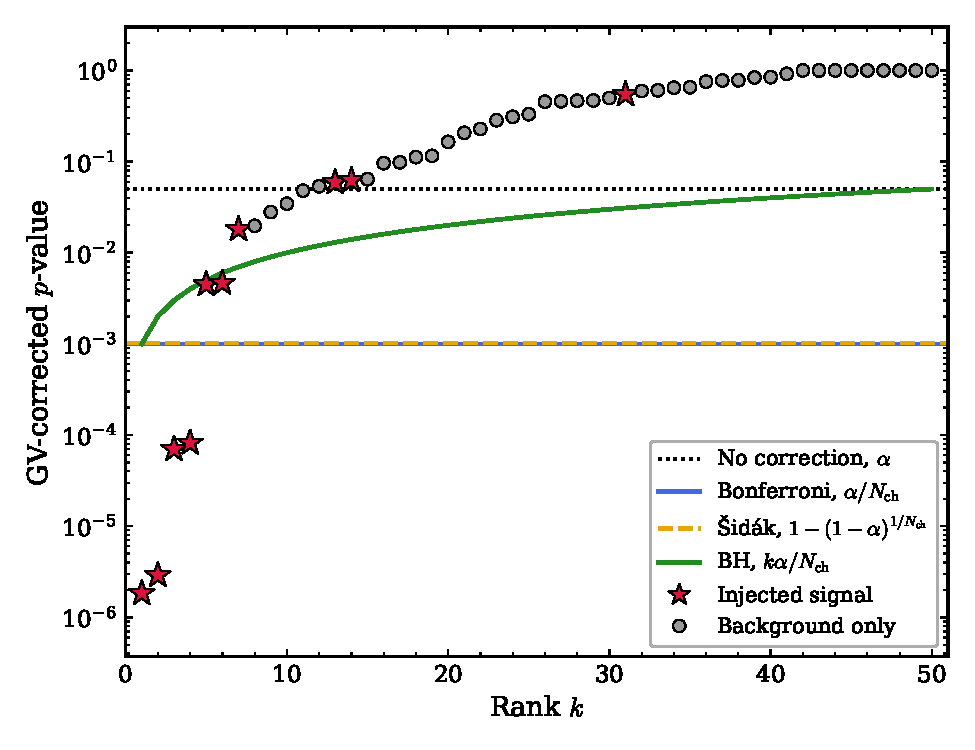
\includegraphics[width=0.49\textwidth]{figures/gg/screening_thresholds.pdf}\hfill
    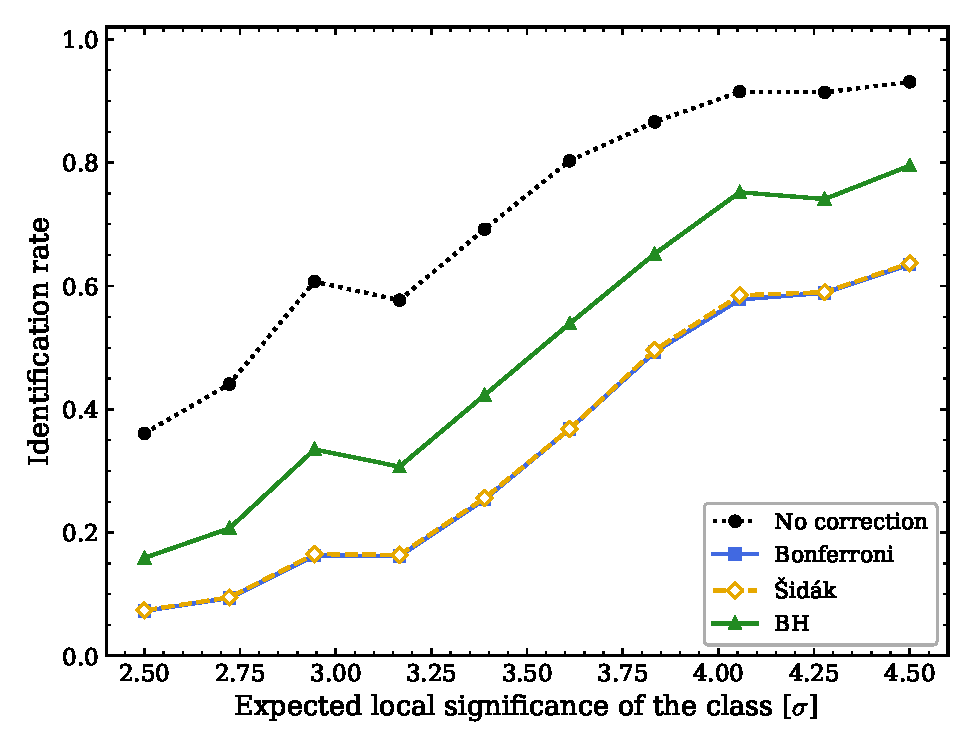
\includegraphics[width=0.49\textwidth]{figures/gg/screening_power.pdf}
    \caption{Screening of $50$ event classes, $10$ of which contain a signal. Left: GV-corrected global $p$-values of the $50$ classes in one pseudo-experiment, sorted in increasing order, with the per-class thresholds without correction ($\alpha=0.05$), with the Bonferroni and \v{S}id\'ak corrections, which coincide on this scale, and the BH threshold $k\alpha/N_\text{ch}$. Stars mark classes with an injected signal, and circles background-only classes. Right: fraction of $1000$ pseudo-experiments in which each signal class is identified, as a function of its expected local significance, for each procedure.}
    \label{fig:screening}
\end{figure}

\begin{table}[htbp]
  \centering
  \caption{Error rates and average number of selected classes of the multiple-testing procedures at $\alpha=0.05$, from $1000$ pseudo-experiments of the screening example with $N_\text{ch}=50$ classes, $10$ of which contain a signal. The statistical uncertainties are at most $0.013$ on the FWER and $0.005$ on the FDR.}
  \label{tab:screening_rates}
  \begin{tabular}{lcccc}
    \toprule
    Procedure & FWER & FDR & \multicolumn{2}{c}{Selected classes} \\
    \cmidrule(lr){4-5}
     & & & signal & background \\
    \midrule
    No correction & 0.853 & 0.199 & 7.11 & 1.92 \\
    Bonferroni & 0.041 & 0.011 & 3.41 & 0.04 \\
    \v{S}id\'ak & 0.042 & 0.011 & 3.43 & 0.04 \\
    BH & 0.209 & 0.037 & 4.91 & 0.25 \\
    \bottomrule
  \end{tabular}
\end{table}
